% !TEX spellcheck = en_US



% ~~~~~~~~~~~~~~~~~~~~~~~~~~~~~~~~~~~~~~~ V
% (NC) 2024Haluk Bingol
% github.com/halukbingol/LaTeX-Templates
%
% Licensees may copy, distribute, display, and perform the work and make derivative works 
% and remixes based on it only for non-commercial purposes. 
% ~~~~~~~~~~~~~~~~~~~~~~~~~~~~~~~~~~~~~~~ A




%\documentclass{beamer}
\documentclass[10pt]{beamer}
	\usetheme{Dresden}
%	\usetheme{Copenhagen}
%	\usetheme{Marburg}
%	\usetheme{CambridgeUS}
%	\usetheme{Warsaw}
%	\usetheme{AnnArbor}

%	\usecolortheme{orchid}
	
%	\usecolortheme{}
%	\useinnertheme{}
%	\useoutertheme{}
%	\setbeamertemplate{bibliography item}[text]
\usepackage{beamerthemesplit}
%\usecolortheme{default}
%\usecolortheme{structure}
%\usepackage{beamerthemesplit} // Activate for custom appearance

\useoutertheme{split}
\usecolortheme{whale}
\useinnertheme{rounded} 
\usecolortheme{orchid}
\setbeamertemplate{blocks}[rounded]




% ~~~~~~~~~~~~~~~~~~~~~~~~~~~~~~~~~~~~~~~ V HB lib
\usepackage{../hbcommon/hbdatastructures} 
\usepackage{../hbcommon/hbpresentation} 
% ~~~~~~~~~~~~~~~~~~~~~~~~~~~~~~~~~~~~~~~ A




% ~~~~~~~~~~~~~~~~~~~~~~~~~~~~~~~~~~~~~~~ V specific	

\usepackage{subcaption} % subfigure

\usepackage[normalem]{ulem} %strikethroug

\usepackage{tikz-qtree} % tree
\usepackage{adjustbox} % tikzpicture alignment

%\usepackage{moreverb} % tab control
\usepackage{fancyvrb} % tab

\usepackage{epstopdf} % eps 2 pdf
\epstopdfsetup{update} % only regenerate pdf files when eps file is newer

% https://tex.stackexchange.com/questions/118173/how-to-write-ceil-and-floor-in-latex
\usepackage{mathtools}
\DeclarePairedDelimiter\ceil{\lceil}{\rceil}
\DeclarePairedDelimiter\floor{\lfloor}{\rfloor}

\newcommand{\hDummy}{dummy}


%\usetikzlibrary{circuits.ee.IEC} % ground symbol
%\newcommand\hGround{%
%	\mathbin{\text{\begin{tikzpicture}[circuit ee IEC,yscale=0.6,xscale=0.5]
%	\draw (0,2ex) to (0,0) node[ground,rotate=-90,xshift=.65ex] {};
%	\end{tikzpicture}}}%
%}

%% https://tex.stackexchange.com/questions/127641/how-do-i-typeset-the-ground-symbol-in-latex
%\DeclareUnicodeCharacter{23DA}{\hGround}
%\DeclareRobustCommand\hGround{%
%	\unskip\nobreak\thinspace\textemdash\allowbreak\thinspace\ignorespaces%
%}



% beamer blocks
% https://tex.stackexchange.com/questions/347269/different-colors-for-different-types-of-blocks-in-beamer
% https://tex.stackexchange.com/questions/28760/custom-beamer-blocks-for-pros-and-cons/

% https://tex.stackexchange.com/questions/1858/stable-vertical-alignment-of-columns-in-beamer
% https://tex.stackexchange.com/questions/127027/vertical-alignment-of-tikz-picture-in-a-table-cell
% https://tex.stackexchange.com/questions/172434/drawing-vertical-hierarchical-n-ary-tree-in-tikz
%  ~~~~~~~~~~~~~~~~~~~~~~~~~~~~~~~~~~~~~~~ A




% ~~~~~~~~~~~~~~~~~~~~~~~~~~~~~~~~~~~~~~~ V
%	\newcommand{\hAbs}[1]{\ensuremath{\left \lvert \, #1 \, \right \rvert} } % |x|
%	\newcommand{\hMean}[1]{\ensuremath{<\!\! #1 \!\!>}} % average
%	\newcommand{\hMean}[1]{\ensuremath{\overline{#1}}}
% ~~~~~~~~~~~~~~~~~~~~~~~~~~~~~~~~~~~~~~~ A


%: ==== HB Header Common Packages v20160423 ====V
	\usepackage[utf8]{inputenc} % To use Unicode characters
	\usepackage[iso]{datetime}
	%	\usepackage{etex}
	
%	\usepackage[a4paper]{geometry}
	
	\usepackage{xcolor}
	% black, blue, brown, cyan, darkgray, gray, green, lightgray, lime, 
	% magenta, olive, orange, pink, purple, red, teal, violet, white, yellow
%	\usepackage[colorlinks=true,linkcolor=red,urlcolor=blue,citecolor=red]%
%		{hyperref}
	\usepackage{graphicx,epstopdf}
	% \graphicspath{{fig}}
%	\graphicspath{{../common/figures/}}
	% \DeclareGraphicsExtensions{.pdf,.jpeg,.png,.eps}
	% \DeclareGraphicsRule{.tif}{png}{.png}%
	%	{`convert #1 `dirname #1`/`basename #1 .tif`.png}
%	\usepackage{subfigure}
%\usepackage{subfig}
%\usepackage{subcaption}
% ~~~~~~~~~~~~~~~~~~~~~~~~~~~~~~~~~~~~~~~ V HB Header Common Packages v20160423 




% ~~~~~~~~~~~~~~~~~~~~~~~~~~~~~~~~~~~~~~~ V
\title{
	cis112\\
	Tree- Heap
}

\author[Bingol]{Haluk O. Bingol}

\institute{
	Faculty of Computer and Information Sciences\\
	Yeditepe University
}

%\date{
%	cis112\\ 
%	Yeditepe University, 2024-02-25
%}
\date{
	{\tiny v2024-05-12}
}
% ~~~~~~~~~~~~~~~~~~~~~~~~~~~~~~~~~~~~~~~ A



\begin{document}
% ~~~~~~~~~~~~~~~~~~~~~~~~~~~~~~~~~~~~~~~ 




% ~~~~~~~~~~~~~~~~~~~~~~~~~~~~~~~~~~~~~~~ V Title
\frame{\titlepage}
% ~~~~~~~~~~~~~~~~~~~~~~~~~~~~~~~~~~~~~~~ A 




% ~~~~~~~~~~~~~~~~~~~~~~~~~~~~~~~~~~~~~~~ V Content
\begin{frame}[t]\frametitle{Content}
	\begin{columns}[T]
	\begin{column}{.5\linewidth}   
	    	\tableofcontents[hideallsubsections]
		
		\hCite{ %
	\cite{knuth1973artv1}, %
	\cite{cormen2022introduction}, %
	\cite{preiss1999}, %
	\cite{aho1974design}, %
	\cite{horowitz1982fundamentals}, %
	\cite{horstmann2016big}, %
	\cite{grimaldi2006discrete}
}
	\end{column}
	\begin{column}{.5\linewidth}
		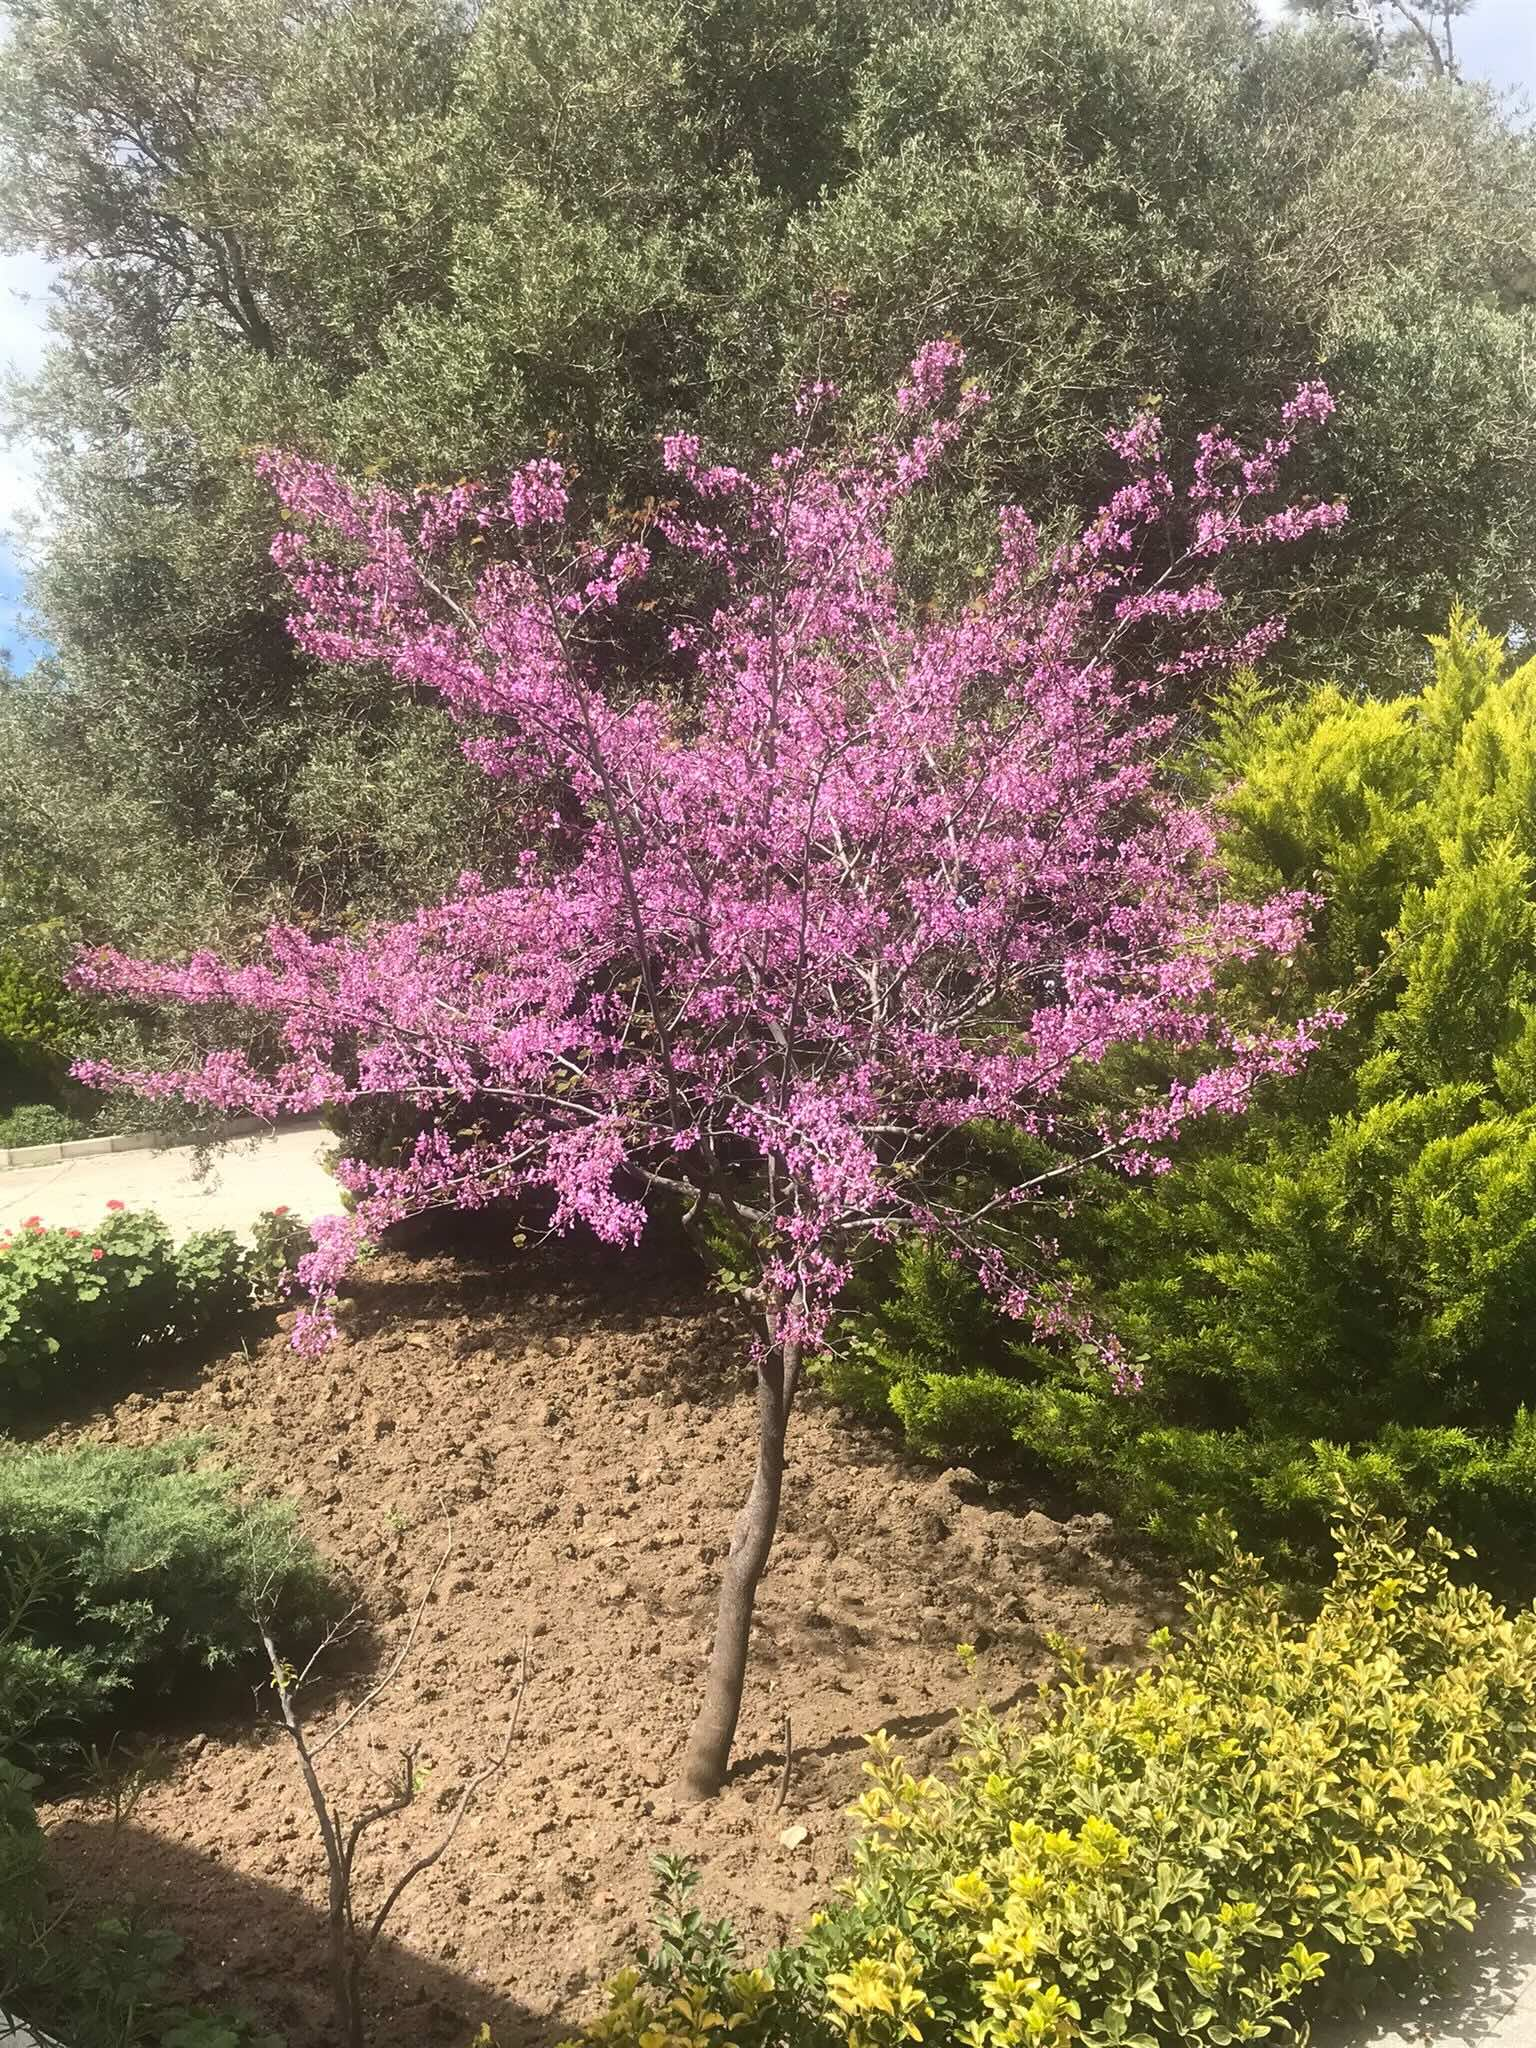
\includegraphics[width=.8\columnwidth]
		{fig/fig-Erguvan.jpg}
%		{example-image}
	\end{column}
	\end{columns}
\end{frame}
% ~~~~~~~~~~~~~~~~~~~~~~~~~~~~~~~~~~~~~~~ A




% ~~~~~~~~~~~~~~~~~~~~~~~~~~~~~~~~~~~~~~ V
\hSection{Motivation}{Hierarchy}{}
% ~~~~~~~~~~~~~~~~~~~~~~~~~~~~~~~~~~~~~~ A




% ~~~~~~~~~~~~~~~~~~~~~~~~~~~~~~~~~~~~~~ V
\hSection{Definitions}{}{\hCite{ %
	\cite{knuth1973artv1}, %
	\cite{cormen2022introduction}, %
	\cite{preiss1999}, %
	\cite{aho1974design}, %
	\cite{horowitz1982fundamentals}, %
	\cite{horstmann2016big}, %
	\cite{grimaldi2006discrete}
}}
% ~~~~~~~~~~~~~~~~~~~~~~~~~~~~~~~~~~~~~~ A




\subsection{Balanced Binary Trees}
% ~~~~~~~~~~~~~~~~~~~~~~~~~~~~~~~~~~~~~~ V
\begin{frame}[t]\frametitle{Balanced Binary Trees}
	\vspace{-0.5cm}
	\begin{columns}[T] % >>>>
	\begin{column}{.5\linewidth} % ++++ V
		\begin{definition}
			 A binary tree $T = \{ r, T_{l}, T_{r} \}$ is \hDefined{balanced} 
			 iff
			\begin{itemize}
			
				\item
				$T$ is empty or
			
				\item
				$T_{l}, T_{r}$ have ``almost the same height''.
			\end{itemize}		 
		\end{definition}
		
		\textbf{Remark.}
		\begin{itemize}
			
			\item 
			Consider ``almost the same height'' as difference of 1.

			\item			
			How to \hEmph{keep a tree balanced} is an important issue that 
			we will deal with

		\end{itemize}
		
	\end{column} % ++++ A
	\begin{column}{.5\linewidth} % ++++ V
		\begin{example}
		{\scriptsize
			\begin{figure}[htbp]
			\begin{center}
				\begin{tikzpicture}
	\tikzset{every leaf node/.style={font=\sffamily}}
	\Tree
	[.$1$
		[.$2$
			[.$4$ 
				[.$8$ ]
				[.$9$ ]
			]
			[.$5$
				[.$10$ ]
				[.$11$ ]				
			]
		]
		[.$3$
			[.$6$ ]
			[.$7$ ]
		]
	]
\end{tikzpicture}

			\end{center}
			\end{figure}
		} % fsize
		\end{example}
	\end{column} % ++++ A
	\end{columns} % <<<<
\end{frame}
% ~~~~~~~~~~~~~~~~~~~~~~~~~~~~~~~~~~~~~~ A



\subsection{Heap}
% ~~~~~~~~~~~~~~~~~~~~~~~~~~~~~~~~~~~~~~ V
\begin{frame}[t]\frametitle{Max-Heap Property}

	\vspace{-0.5cm}
	\begin{columns}[T] % >>>>
	\begin{column}{.5\linewidth} % ++++ V
%	{\footnotesize 
		\begin{definition}
			An binary tree  \hCode{T} has  \hDefined{Max-Heap Property} 
			iff
			\[
				\hCode{i.parent.key $\ge$ i.key} 
			\]
			for all nodes $i$.
			
			A binary tree with max-heap property is called \hDefined{max-heap}.
		\end{definition}
		
%	} %fsize
	\end{column} % ++++ A
	\begin{column}{.5\linewidth} % ++++ V
		\begin{example}
		{\scriptsize
		\begin{figure}[htbp]
		\begin{center}
			\begin{tikzpicture}
	\tikzset{every leaf node/.style={font=\sffamily}}
	\Tree
	[.\hIndex{1}$16$
		[.\hIndex{2}$14$
			[.\hIndex{4}$8$ 
				[.\hIndex{8}$2$ ]
				[.\hIndex{9}$4$ ]
			]
			[.\hIndex{5}$7$
				[.\hIndex{10}$1$ ]
				[.$~$ ]				
			]
		]
		[.\hIndex{3}$10$
			[.\hIndex{6}$9$ ]
			[.\hIndex{7}$3$ ]
		]
	]
\end{tikzpicture}

		\end{center}
		\end{figure}
		} % fsize


		{\tiny 
			\begin{table}[t]
			\setlength{\tabcolsep}{5pt}
			\begin{tabular}
				{|
					p{.3cm} 
					!{\vrule width 1pt}
					*{10}{p{.05cm}|} 
				}
				\hline
				\textcolor{colorIndex}{index}	&\textcolor{colorIndex}{1}	&\textcolor{colorIndex}{2}	&\textcolor{colorIndex}{3}	&\textcolor{colorIndex}{4}	&\textcolor{colorIndex}{5}	&\textcolor{colorIndex}{6}	&\textcolor{colorIndex}{7}	&\textcolor{colorIndex}{8}	&\textcolor{colorIndex}{9}	&\textcolor{colorIndex}{10}\\
				\noalign{\hrule height 1pt}
				Value	&16	&14	&10	&8	&7	&9	&3	&2	&4	&1\\
				\hline
			\end{tabular}
			\end{table}
		} % fsize

		\end{example}

	\end{column} % ++++ A
	\end{columns} % <<<<
\end{frame}
% ~~~~~~~~~~~~~~~~~~~~~~~~~~~~~~~~~~~~~~ A



\section{Priority Queue}
% ~~~~~~~~~~~~~~~~~~~~~~~~~~~~~~~~~~~~~~ V
\begin{frame}[t]\frametitle{Priority Queue}

	\vspace{-0.5cm}
	\begin{columns}[T] % >>>>
	\begin{column}{.6\linewidth} % ++++ V
%	{\footnotesize 
		\begin{definition}[Mathematical]
			A \hDefined{priority queue}  is a data structure of 
			a set \hEmph{\(S\)} of elements \hEmph{\(x\)},
			each has a key \hCode{x.key}.
			
			A \hDefined{max-priority queue} has the following operations
			\begin{enumerate}
			
				\item 
				\hEmph{\hCode{insert(S, x)} }inserts the element \hCode{x}
				
				\item 
				\hEmph{\hCode{maximum(S)}} returns the element of \hCode{S} 
				with the largest \hCode{key}
				
				\item 
				\hEmph{\hCode{extractMax(S)}} removes and returns the element of \hCode{S} 
				with the largest \hCode{key}
			\end{enumerate}			
		\end{definition}
		
		\textbf{Q.}
		What happens if there are more than one element with  the largest \hCode{key}?
		
%	} %fsize
	\end{column} % ++++ A
	\begin{column}{.4\linewidth} % ++++ V
		\begin{example}
		{\scriptsize
%			\begin{tabular}{c c c}
	\adjustbox{valign=t}{			
		\begin{tikzpicture}
			\tikzset{every leaf node/.style={font=\sffamily}}
			\Tree
			[.{A} ]
		\end{tikzpicture}
	} % \adjustbox
	&
	\adjustbox{valign=t}{	
		\begin{tikzpicture}
			\tikzset{every leaf node/.style={font=\sffamily}}
			\Tree
			[.{B} 
				[.{C} ]
			]
		\end{tikzpicture}
	} % \adjustbox
	&
	\adjustbox{valign=t}{	
		\begin{tikzpicture}
			\tikzset{every leaf node/.style={font=\sffamily}}
			\Tree
			[.{0}
				[.$1$
					[.$3$  ]
					[.$4$  ]
					[.$5$  ]
				]
				[.$2$
					[.$6$ ]
					[.$7$ 
						[.$8$ ]
						[.$9$ ]
					]
				]
			]
		\end{tikzpicture}
	} % \adjustbox
\end{tabular}

		} % fsize
		\end{example}

	\end{column} % ++++ A
	\end{columns} % <<<<
\end{frame}
% ~~~~~~~~~~~~~~~~~~~~~~~~~~~~~~~~~~~~~~ A




% ~~~~~~~~~~~~~~~~~~~~~~~~~~~~~~~~~~~~~~ V
\hSection{Implementation}{}{}
% ~~~~~~~~~~~~~~~~~~~~~~~~~~~~~~~~~~~~~~ A




% ~~~~~~~~~~~~~~~~~~~~~~~~~~~~~~~~~~~~~~ V
\begin{frame}[t]\frametitle{Array-Like Approach}

%	\vspace{-0.5cm}
	\begin{columns}[T] % >>>>
	\begin{column}{.5\linewidth} % ++++ V
	{\footnotesize
	    	A heap can be implemented as an array (array-like structures).
		
		For node at index \(i\)
			
		\begin{itemize}
			\item
			Starting index 1, 
			i.e., not using index 0
			\begin{itemize}
				\item
				 \( parent = \floor*{i / 2} \)
				
				\item
				\( left = 2 i \)
				
				\item
				\( right = 2 i + 1 \)
			\end{itemize}
			
			\item
			Using index 0
			\begin{itemize}
				\item
				 \( parent = \floor*{ (i - 1) / 2} \)
				
				\item
				\( left = 2 i + 1 \)
				
				\item
				\( right = 2 i + 2 \)
			\end{itemize}
		\end{itemize}
	} % fsize
	\end{column} % ++++ A
	\begin{column}{.5\linewidth} % ++++ V
		\begin{example}
		{\footnotesize
		Starting at index 1.
		} %fsize

		{\scriptsize
			\begin{tikzpicture}
	\tikzset{every leaf node/.style={font=\sffamily}}
	\Tree
	[.\hIndex{1}$1$
		[.\hIndex{2}$2$
			[.\hIndex{4}$4$ 
				[.\hIndex{8}$8$ ]
				[.\hIndex{9}$9$ ]
			]
			[.\hIndex{5}$5$
				[.\hIndex{10}$10$ ]
				[.\hIndex{11}$11$ ]				
			]
		]
		[.\hIndex{3}$3$
			[.\hIndex{6}$6$
				[.\hIndex{12}$12$ ]
				[.\hIndex{13}$13$ ]
			]
			[.\hIndex{7}$7$ 
				[.\hIndex{14}$14$ ]
				[.\hIndex{15}$15$ ]
			]
		]
	]
\end{tikzpicture}

		} %fsize

		{\tiny 
			\begin{table}[t]
			\setlength{\tabcolsep}{5pt}
			\begin{tabular}
				{|
					p{.3cm} 
					!{\vrule width 1pt}
					*{11}{p{.05cm}|} 
				}
				\hline
				\textcolor{colorIndex}{index}	
				&\textcolor{red}{0}
				&\textcolor{colorIndex}{1}	&\textcolor{colorIndex}{2}	
				&\textcolor{colorIndex}{3}	&\textcolor{colorIndex}{4}	
				&\textcolor{colorIndex}{5}	&\textcolor{colorIndex}{6}	
				&\textcolor{colorIndex}{7}	&\textcolor{colorIndex}{8}	
				&\textcolor{colorIndex}{9}	&\textcolor{colorIndex}{...}\\
				
				\noalign{\hrule height 1pt}
				
				Value	
				&\textcolor{red}{$\times$}	
				&1	&2	&3	&4	&5	&6	&7	&8	&9	&...\\
				\hline
			\end{tabular}
			\end{table}
		} % fsize
		\end{example}
	\end{column} % ++++ A
	\end{columns} % <<<<
\end{frame}
% ~~~~~~~~~~~~~~~~~~~~~~~~~~~~~~~~~~~~~~ A




% ~~~~~~~~~~~~~~~~~~~~~~~~~~~~~~~~~~~~~~ V
\begin{frame}[t]\frametitle{``left-justified''}
	\begin{columns}[T] % >>>>
	\begin{column}{.5\linewidth} % ++++ V
	    	
		\begin{itemize}
			\item
			Use array-like implementation.
			
			\item
			For a tree with \( N \) nodes,
			use indices \(1, 2, \dotsc, N \)
		\end{itemize}
	\end{column} % ++++ A
	\begin{column}{.5\linewidth} % ++++ V
		\begin{example}
		{\footnotesize
		Starting at index 1.
		} %fsize

		{\scriptsize
			\begin{tikzpicture}
	\tikzset{every leaf node/.style={font=\sffamily}}
	\Tree
	[.\hIndex{1}$1$
		[.\hIndex{2}$2$
			[.\hIndex{4}$4$ 
				[.\hIndex{8}$8$ ]
				[.\hIndex{9}$9$ ]
			]
			[.\hIndex{5}$5$
				[.\hIndex{10}$10$ ]
				[.\hIndex{11}$11$ ]				
			]
		]
		[.\hIndex{3}$3$
			[.\hIndex{6}$6$
				[.\hIndex{12}$12$ ]
				[.\hIndex{13}$13$ ]
			]
			[.\hIndex{7}$7$ 
				[.\hIndex{14}$14$ ]
				[.\hIndex{15}$15$ ]
			]
		]
	]
\end{tikzpicture}

		} %fsize

		{\tiny 
			\begin{table}[t]
			\setlength{\tabcolsep}{5pt}
			\begin{tabular}
				{|
					p{.3cm} 
					!{\vrule width 1pt}
					*{11}{p{.05cm}|} 
				}
				\hline
				\textcolor{colorIndex}{index}	
				&\textcolor{red}{0}
				&\textcolor{colorIndex}{1}	&\textcolor{colorIndex}{2}	
				&\textcolor{colorIndex}{3}	&\textcolor{colorIndex}{4}	
				&\textcolor{colorIndex}{5}	&\textcolor{colorIndex}{6}	
				&\textcolor{colorIndex}{7}	&\textcolor{colorIndex}{8}	
				&\textcolor{colorIndex}{9}	&\textcolor{colorIndex}{...}\\
				
				\noalign{\hrule height 1pt}
				
				Value	
				&\textcolor{red}{$\times$}	
				&1	&2	&3	&4	&5	&6	&7	&8	&9	&...\\
				\hline
			\end{tabular}
			\end{table}
		} % fsize
		\end{example}
		\end{column} % ++++ A
	\end{columns} % <<<<
\end{frame}
% ~~~~~~~~~~~~~~~~~~~~~~~~~~~~~~~~~~~~~~ A




% ~~~~~~~~~~~~~~~~~~~~~~~~~~~~~~~~~~~~~~ V
\begin{frame}[t]\frametitle{Observations}
	\begin{columns}[T] % >>>>
	\begin{column}{.5\linewidth} % ++++ V
	    	
		\begin{itemize}
			\item
			\hEmph{insert} a new node $x$ at  the first available location,
			e.g., index 14
			
			\item
			\hEmph{remove} a node,
			the first available location becomes one less index (move to the left),
			e.g., 	index 13 becomes empty
		\end{itemize}
	\end{column} % ++++ A
	\begin{column}{.5\linewidth} % ++++ V
		\begin{example}
		{\footnotesize
		Starting at index 1.
		} %fsize

		{\scriptsize
			\begin{tikzpicture}
	\tikzset{every leaf node/.style={font=\sffamily}}
	\Tree
	[.\hIndex{1}$$
		[.\hIndex{2}$2$
			[.\hIndex{4}$4$ 
				[.\hIndex{8}$8$ ]
				[.\hIndex{9}$9$ ]
			]
			[.\hIndex{5}$5$
				[.\hIndex{10}$10$ ]
				[.\hIndex{11}$11$ ]				
			]
		]
		[.\hIndex{3}$3$
			[.\hIndex{6}$6$
				[.\hIndex{12}$12$ ]
				[.\hIndex{13}$13$ ]
			]
			[.\hIndex{7}$$ 
				[.\hIndex{14}$$ ]
				[.\hIndex{15}$$ ]
			]
		]
	]
\end{tikzpicture}

		} %fsize

		{\tiny 
			\begin{table}[t]
			\setlength{\tabcolsep}{5pt}
			\begin{tabular}
				{|
					p{.3cm} 
					!{\vrule width 1pt}
					*{11}{p{.05cm}|} 
				}
				\hline
				\textcolor{colorIndex}{index}	
				&\textcolor{red}{0}
				&\textcolor{colorIndex}{1}	&\textcolor{colorIndex}{2}	
				&\textcolor{colorIndex}{3}	&\textcolor{colorIndex}{4}	
				&\textcolor{colorIndex}{5}	&\textcolor{colorIndex}{6}	
				&\textcolor{colorIndex}{7}	&\textcolor{colorIndex}{8}	
				&\textcolor{colorIndex}{9}	&\textcolor{colorIndex}{...}\\
				
				\noalign{\hrule height 1pt}
				
				Value	
				&\textcolor{red}{$\times$}	
				&1	&2	&3	&4	&5	&6	&7	&8	&9	&...\\
				\hline
			\end{tabular}
			\end{table}
		} % fsize
		\end{example}
		\end{column} % ++++ A
	\end{columns} % <<<<
\end{frame}
% ~~~~~~~~~~~~~~~~~~~~~~~~~~~~~~~~~~~~~~ A




% ~~~~~~~~~~~~~~~~~~~~~~~~~~~~~~~~~~~~~~ V
\begin{frame}[t]\frametitle{Insert}
	Insert $95$ to the first available location (FAL) and move it up
	
	\begin{figure}[htbp]
	\begin{center}

	\begin{subfigure}[b]{0.45\textwidth}
		\centering
		\only<1-2>{
			Initial State. FAL is in the left of 37
			\includegraphics[width=\textwidth]
				{fig/fig-bst-insert-95-01.pdf}
		}
		\only<3-4>{
			Swap 95 with 37
			\includegraphics[width=\textwidth]
				{fig/fig-bst-insert-95-03.pdf}
		}
		\only<5-6>{
			Swap 95 with82
			\includegraphics[width=\textwidth]
				{fig/fig-bst-insert-95-05.pdf}
		}
	\end{subfigure}

	\hfill

	\begin{subfigure}[b]{0.45\textwidth}
		\centering
		\only<2-3>{
			Insert 95 in FAL
			\includegraphics[width=\textwidth]
				{fig/fig-bst-insert-95-02.pdf}
		}
		\only<4-5>{
			Swap 95 with 51
			\includegraphics[width=\textwidth]
				{fig/fig-bst-insert-95-04.pdf}
		}
	\end{subfigure}

	\end{center}
	\end{figure}
	
\end{frame}
% ~~~~~~~~~~~~~~~~~~~~~~~~~~~~~~~~~~~~~~ A




% ~~~~~~~~~~~~~~~~~~~~~~~~~~~~~~~~~~~~~~ V
\begin{frame}[t]\frametitle{Delete}
	Delete the root, move the last node to the root and move it down
	
	\begin{figure}[htbp]
	\begin{center}
		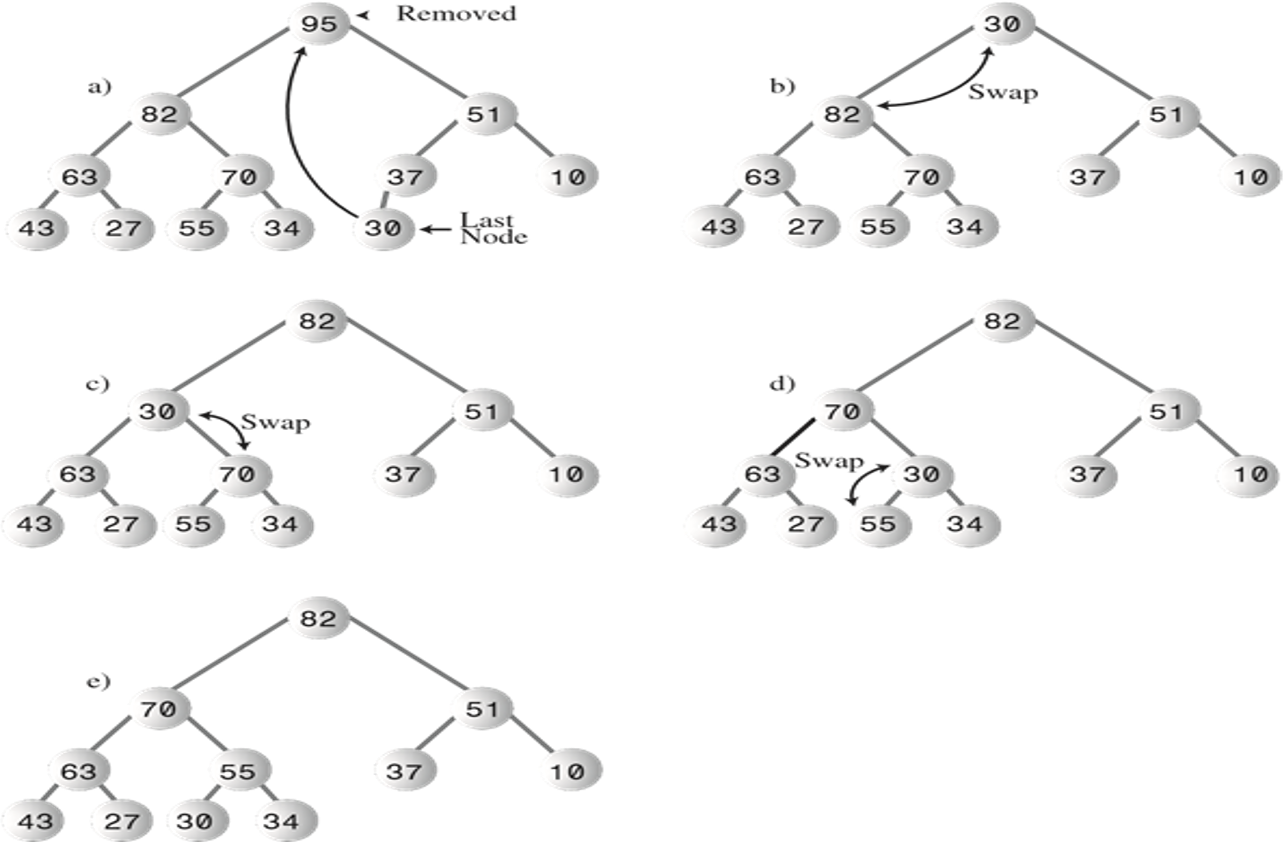
\includegraphics[width=.9\columnwidth]
		{fig/fig-heap-remove.png}
		\hCite{%
			\cite{lafore2003data}%
		}
	\end{center}
	\end{figure}
\end{frame}
% ~~~~~~~~~~~~~~~~~~~~~~~~~~~~~~~~~~~~~~ A




% ~~~~~~~~~~~~~~~~~~~~~~~~~~~~~~~~~~~~~~ V
\begin{frame}[t]\frametitle{Heapsort}
	\begin{figure}[htbp]
	\begin{center}
		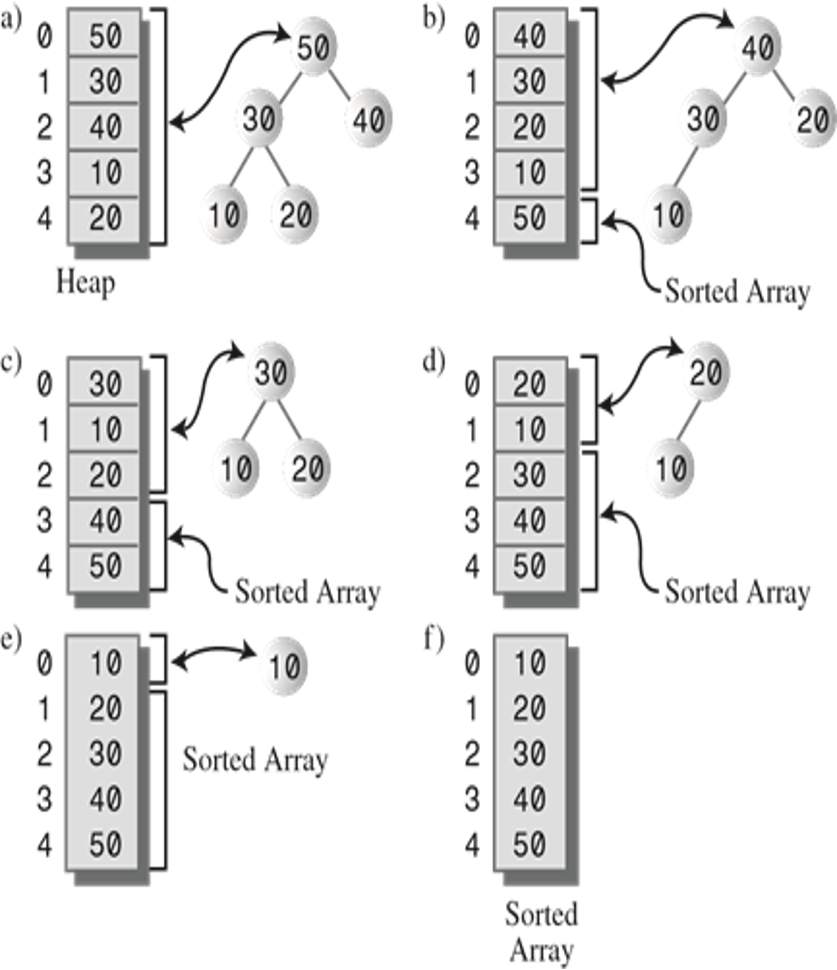
\includegraphics[width=.5\columnwidth]
		{fig/fig-heapsort.png}
		\hCite{%
			\cite{lafore2003data}%
		}
	\end{center}
	\end{figure}
\end{frame}
% ~~~~~~~~~~~~~~~~~~~~~~~~~~~~~~~~~~~~~~ A




% ~~~~~~~~~~~~~~~~~~~~~~~~~~~~~~~~~~~~~~ V References bib
\begin{frame}[t,allowframebreaks]\frametitle{References}
	\setbeamertemplate{bibliography item}[text] % sets numbers in references
%	\bibliographystyle{abbrv}
%	\bibliographystyle{apalike}
%	\bibliographystyle{ieeetr}
	\bibliographystyle{IEEEtran}
	%
	\tiny\bibliography{../hbcommon/bingol-DataStructures} % bib file

	
\end{frame}
% ~~~~~~~~~~~~~~~~~~~~~~~~~~~~~~~~~~~~~~ A

% ~~~~~~~~~~~~~~~~~~~~~~~~~~~~~~~~~~~~~~~ 
\end{document}
